\section{Thermal shield vibrations}\label{sec:5:thermal-vibrations}
A spherical plate with radius $r_s$ that is fixed at the edge can vibrate in different vibrational modes labeled by the indices $(k,l)$, where $k \in [1,\infty)$ and $l \in [0, \infty)$.
The exact vibrational frequency and the mode shape can only be given in terms of the Bessel functions. In fact, one of the first occurrences of these functions can be traced back to Euler trying to solve the very similar problem of a vibrating perfectly flexible membrane \cite{Dutka_1995}.
In general, the vibrations of a plate made out of a real material with thickness $d$ can be described by the differential equation \cite[p. 490]{Rao_2019}
\begin{equation}
  D \nabla^2\nabla^2 u = -\rho d \ddot{u}
\end{equation} 
where $D$ is given by material properties like Youngs module $E$ and the poisson number $\nu$ as
\begin{equation}
  D = \frac{d^3 E}{12(1-\nu^2)} .
\end{equation}
The general solution of this differential equation can be written in terms of the Bessel functions as (derived in Ref. \cite[p. 490-495]{Rao_2019}) 
\begin{equation}
  u_{kl}(r, \theta, t) = \left[J_l(\beta_k r) - \frac{J_l(\beta_k r_s)}{I_l(\beta_k r_s)}I_l(\beta_k r)\right]\cos(l\theta+\phi_1)\sin(\omega_{kl}t+\phi_2)
\end{equation}
with
\begin{equation} \label{eq:5:vibration-frequency}
  \beta_k = \frac{\tilde{r}_k}{r_s} \quad \text{and} \quad \omega_{kl} = \frac{\tilde{r}_k^2}{r_s^2}\sqrt{\frac{D}{\rho d}} = \tilde{r}_k^2\frac{d}{r_s^2}\sqrt{\frac{E}{12\rho(1-\nu^2)}} ,
\end{equation}
where $\tilde{r}_k$ is the $k$-th solution of the equation
\begin{equation}\label{eq:5:bessel-zeros}
  J_l(\tilde{r}_k)I_{l+1}(\tilde{r}_k)+I_l(\tilde{r}_k)J_{l+1}(\tilde{r}_k) = 0 .
\end{equation}
The phases $\phi_1$ and $\phi_2$ can be determined by initial conditions and refer to the rotation of the plate as well as temporal offsets. The shape of the first few modes is shown in \cref{fig:5:vibrational-modes}.
\begin{figure}[!htbp]
  \centering
  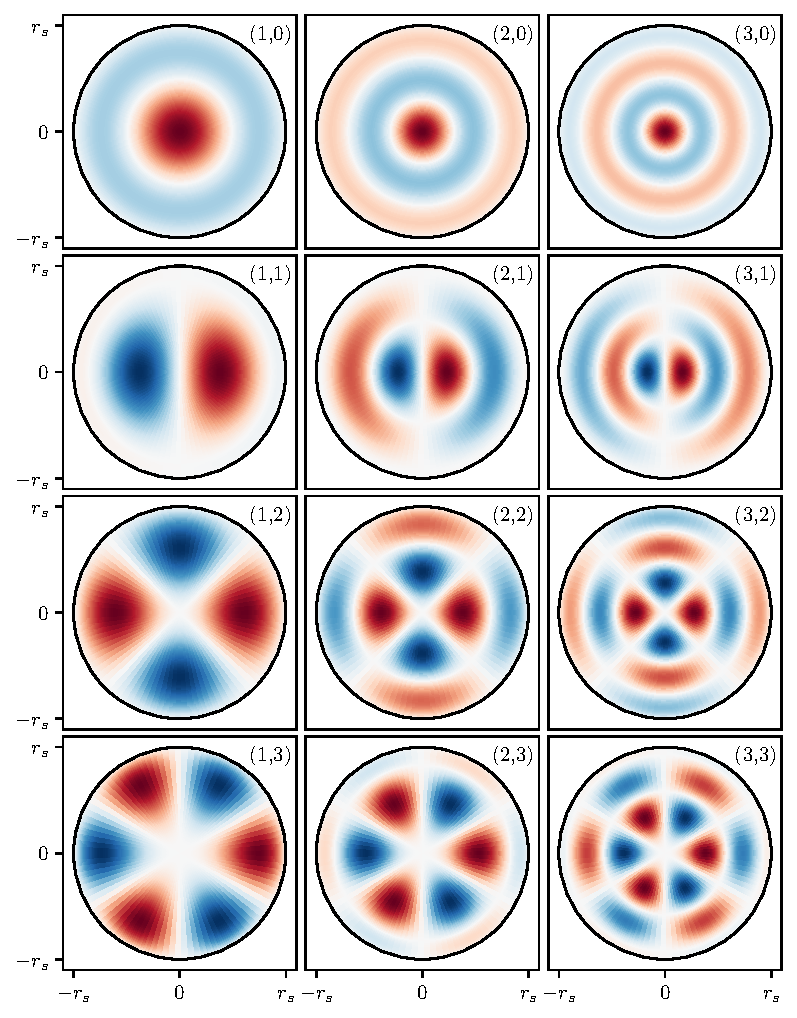
\includegraphics[width=\textwidth]{./../figures/vibrations/vibrational-modes-rd_bu.pdf}
  \caption{Shape of the first 12 modes $(k,l)$ ($k \geq 1$ and $l \geq 0$) of a vibrating spherical plate fixed at the edge with $r_s/d = 1000$.}
  \label{fig:5:vibrational-modes}
\end{figure}
In general, every possible vibration of the plates can be expressed as a sum of these default modes $u_{kl}$.
The amplitude $\op{z}$ of the vibrations are determined by the temperature $T$ and can be calculated by treating the amplitude of each vibration as a separate quantum harmonic oscillator with frequency $\omega_{kl}$.
The expectation value of the amplitude $\avg{z\op{z}}$ is obviously zero and the variance $(\Delta \op{z})^2 = \avg{\op{z}^2} - \avg{\op{z}}^2$ at temperature $T$ is given by (derivation in \cref{apx:thermal-harmonic-oscillator})
\begin{equation}\label{eq:5:amplitude-variance}
  (\Delta \op{z}_{kl})^2_T = \frac{\hbar}{2\tilde{m}\omega_{kl}}\coth(\frac{\hbar \omega_{kl}}{2k_BT}) \approx \frac{k_B T}{\tilde{m}\omega_{kl}^2}
\end{equation}
where in the last step $\hbar\omega \ll k_B T$ was used. $\tilde{m}$ is the \textit{effective mass} of the mode in which the precise shape is considered. A intuitive estimation for this mass can be given by the average amplitude of the mode 
\begin{equation}\label{eq:5:effective-mass}
  \tilde{m} = m\frac{1}{\pi r_s^2}\int\limits_0^{r_s} \dd r \int\limits_0^{2\pi} r\dd\theta \, u_{kl}(r, \theta, t)
\end{equation}
with $m=\rho \pi r_s^2 d$ being the total mass of the shield.
The amplitude of the plate vibrations scale therefore with $\Delta z_{kl} \propto \omega^{-1}$ at high temperatures or for low frequencies.




\subsection*{The effect of infinite modes}
For a shield with radius $r_s = 1\si{cm}$ (in the following referred to as the \q{large shield}) and thickness $d=100\si{nmm}$ made out of Copper with $E = 110\si{GPa}$ and $\nu = 1/3$, the frequencies for the first few modes are between $11.0\si{s^{-1}}$ for $(1,0)$ up to $1018\si{s^{-1}}$ for $(7,6)$.
These frequencies are very low and thus the energy of the vibration $\hbar \omega$ is small compared to the thermal energy $k_B T$ at all reasonable temperatures.
This means, that one expects a lot of modes to be highly populated. Even at temperatures of $10^{-6} \si{K}$, the first $600$ modes are all equally likely to occur with a probability of $\approx 1/Z$ where $Z$ is the partition function
\begin{equation}
  Z = \sum_{m\in\{(k,l)\}} e^{-\beta \hbar \omega_m} .
\end{equation}

It is possible to calculate the asymptotic increase in the frequencies $\omega_{kl}$ for high modes $k \rightarrow \infty$.
This is, because the behavior for large inputs of the Bessel functions \cite[eq. 10.17.3]{DLMF}
\begin{equation}
  J_l(x) \sim \cos(x - \frac{l \pi}{2} - \frac{\pi}{4}) \quad \text{for} \ x \rightarrow \infty
\end{equation}
and modified Bessel functions \cite[eq. 10.40.1]{DLMF}
\begin{equation}
  I_l(x) \sim \frac{e^x}{\sqrt{2\pi x}} \quad \text{for} \ x \rightarrow \infty
\end{equation}
is known resulting in an asymptotic expansion of eq. \eqref{eq:5:bessel-zeros} 
\begin{equation}
  \sim \frac{e^x}{\sqrt{2\pi x}} \left[\cos(x - \frac{l \pi}{2} - \frac{\pi}{4}) + \cos(x - \frac{l \pi}{2} - \frac{3 \pi}{4})\right] = 0 .
\end{equation}
Therefore, the distribution of zeros $\tilde{r}_k$ is periodic for large $k$ as well as for large $l$.
The frequencies increase therefore with $\mathcal{O}(k^2 + l^2)$ for large modes.
The amplitude $\Delta z_\mathrm{kl} \propto 1/\omega$ therefore decreases quadratically with increasing mode order.
Therefore, even if at reasonable temperatures a lot of modes are occupied, the amplitude and thus the effect of each mode decreases for higher modes.
Additionally, because of the consideration of a real vibrating plate, the amplitude of the maximum of the shape $u_{kl}$ decreases for higher modes because the increased number of bulges require more material of the shield limiting the overall amplitude of the vibration even more.
Due to all these effects combined, it is sufficient to only consider the first few modes in all subsequent in numerical calculations.
However the effects of infinity many modes can be estimated asymptotically using the known scaling of $\omega_{kl}$ with increasing modes $(k,l)$.

It is also interesting to consider the scaling of the amplitudes $\Delta z$ for differently sized shields. 
According to eq. \eqref{eq:5:vibration-frequency}, the frequency $\omega$ increases quadratically with decreasing shield radius $r_s$.
However, the effective mass $\tilde{m}$ eq. \eqref{eq:5:effective-mass} depends also quadratically on the size of the shield resulting in a total dependence of $\Delta z \sim r_s$ for large temperatures and/or low modes.



% \subsection{OLDDD}


% \begin{equation}
%   \op{H} = \hbar \omega \left(\op{a}^\dagger\op{a} + \frac{1}{2}\right) + \tilde{g}_A(\op{z}) \ketbra{\psi_A} + \tilde{g}_B(\op{z}) \ketbra{\psi_B}
% \end{equation}

% Solution:
% \begin{equation}
%   \rho(t) = \frac{1}{2}\begin{pmatrix}
%     1 & e^{-i\varphi(t)}e^{-\gamma(t)}\\
%     e^{i\varphi(t)}e^{-\gamma(t)} & 1
%   \end{pmatrix}
% \end{equation}
% with the phase
% \begin{equation}
%   \varphi(t) = \frac{1}{\hbar^2\omega^2} \left(\sin(\omega t) - \omega t\right) \left(g_A^2 - g_B^2\right)
% \end{equation}
% and the decoherence term
% \begin{equation}
%   \gamma(t) = \frac{4(g_A - g_B)^2}{\hbar^2 \omega^2} \sin^2\left(\frac{\omega t}{2}\right) \left[\bar{n} + \frac{1}{2}\right]
% \end{equation}

% \begin{figure}[!htbp]
%   \centering
%   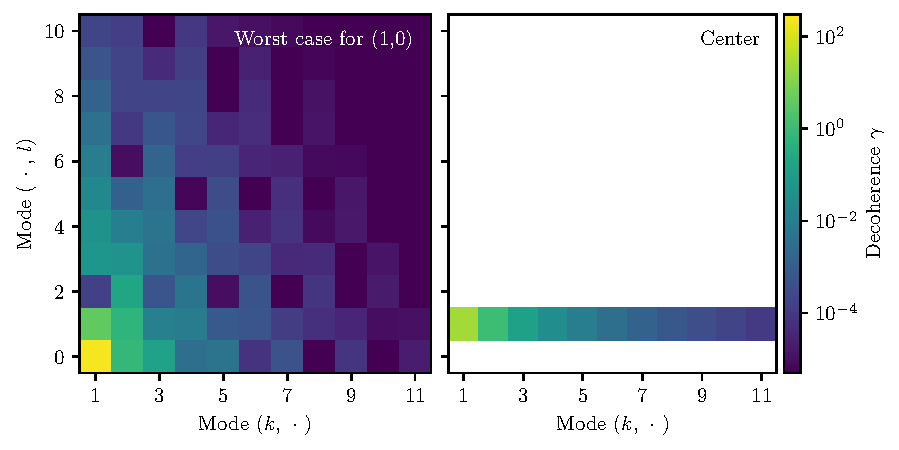
\includegraphics[width=\textwidth]{./../figures/vibrations/decoherence-analytical.pdf}
%   \caption{Maximum decoherence $\gamma$ at $4\si{K}$ for all modes if the cat-state is placed \textbf{left:} at the point with maximum gradient of the mode $(1,0)$ and \textbf{right:} in the center of the plate. It becomes evident, that only a few low modes play an actual role for the total dephasing.}
%   \label{fig:5:}
% \end{figure}


% \begin{figure}[!htbp]
%   \centering
%   \def\svgwidth{\textwidth}
%   \input{./../figures/plate-vibration.pdf_tex}
%   \caption{For a large shield, vibrations can be interpreted locally as if one mass was a distance $\Delta L$ further away from a shield and the other one $\Delta L$ closer and as if both masses would be rotated by an angle $\Delta \theta$.}
% \end{figure}